\chapter{VxWorks 5.5系统镜像的静态二进制注入}

本章介绍如何利用前文所述的
ELF文件二进制插入技术,
实现对VxWorks 5.5系统镜像的注入。
本章由浅入深,
首先分析VxWorks 5.5系统镜像的特殊性,
由此选择合适的技术方案。
在实际的插入工作中,
从实现最简单的插入和劫持开始;
并在后续的插入代码中实现一个简单的
dosFs文件系统监控的功能。
插入完成后,
一旦系统中的程序调用文件系统操作函数(例如read,write),
插入代码将截获这一操作,
并在屏幕上打印相应的信息。


\section{VxWorks 5.5操作系统}

本节主要介绍我们的插入目标———VxWorks 5.5系统镜像。
与介绍ELF插入技术时一样,
我们并不罗列太多的细节,
而是重点讨论与我们的插入工作相关的部分。
本章所有的工作都是围绕vxWorks 5.5展开的,
本章中余下部分提到的VxWorks,
如果没有特别说明,
都是指5.5版本。


\subsection{vxWorks概述}

VxWorks操作系统是美国风河公司旗下的一款嵌入式实时操作系统。
该系统由于其高实时性、高可靠性,在嵌入式实时操作系统领域
占据一席之地,特别是应用于通信、军事、航空航天等
高精尖领域中。

风河公司针对VxWorks推出了一系列开发和调试工具,
以下几项与我们的二进制插入工作有密切关系:

\begin{itemize}
 \item Tornado, 风河公司推出的图形化开发工具,
我们使用该工具创建了可加载的VxWorks系统镜像,
在其基础上进行二进制层面的修改。
 \item FTP Server, 是Tornado自带的FTP程序,
虚拟机利用它从主机中下载VxWorks系统镜像。
 \item Target Server, Tornado自带的目标机调试工具。
可以使用该工具调用正在运行的VxWorks系统中的函数,
从而进行调试。
\end{itemize}


\subsection{VxWorks系统映像种类}

VxWorks的系统映像分为三种类型,
每一种映像类型都对应不同的加载方式。

\begin{itemize}
  \item 可加载的映像类型
\end{itemize}

可引导型映像需要一段引导代码才能装载到RAM中,
然后才能开始执行。


\begin{itemize}
  \item 基于ROM的映像类型,
\end{itemize}

这类镜像首先把自己从ROM或者Flash中
装载到RAM中,然后启动运行。

\begin{itemize}
  \item ROM驻留的映像类型
\end{itemize}

这类镜像与基于ROM的映像类型很相似,
但是它在拷贝自身的时候只拷贝数据段,
代码段仍然驻留在ROM中。
适用于RAM较小的一些嵌入式系统,
但运行速度会比较慢。

我们执行插入的对象是可加载的映像类型。
这类映像本身其实是一个ELF文件,
而不是平坦的二进制文件。
其加载过程由一个加载程序(通常称为bootloader)来完成。



\subsection{可引导型映像的启动流程}

虽然我们的插入工作仅针对ELF文件来进行,
并不修改bootloader的工作方式。
但了解bootloader程序的工作方式是有必要的。
就像在Linux下想要劫持ELF文件调用的共享库,
需要熟悉加载器和动态链接器如何工作一样。

如图\ref{boot}所示,VxWorks可加载型镜像的启动
主要有三个步骤(不考虑bootloader被压缩的情况):

\begin{figure}[h!]
    \centering
    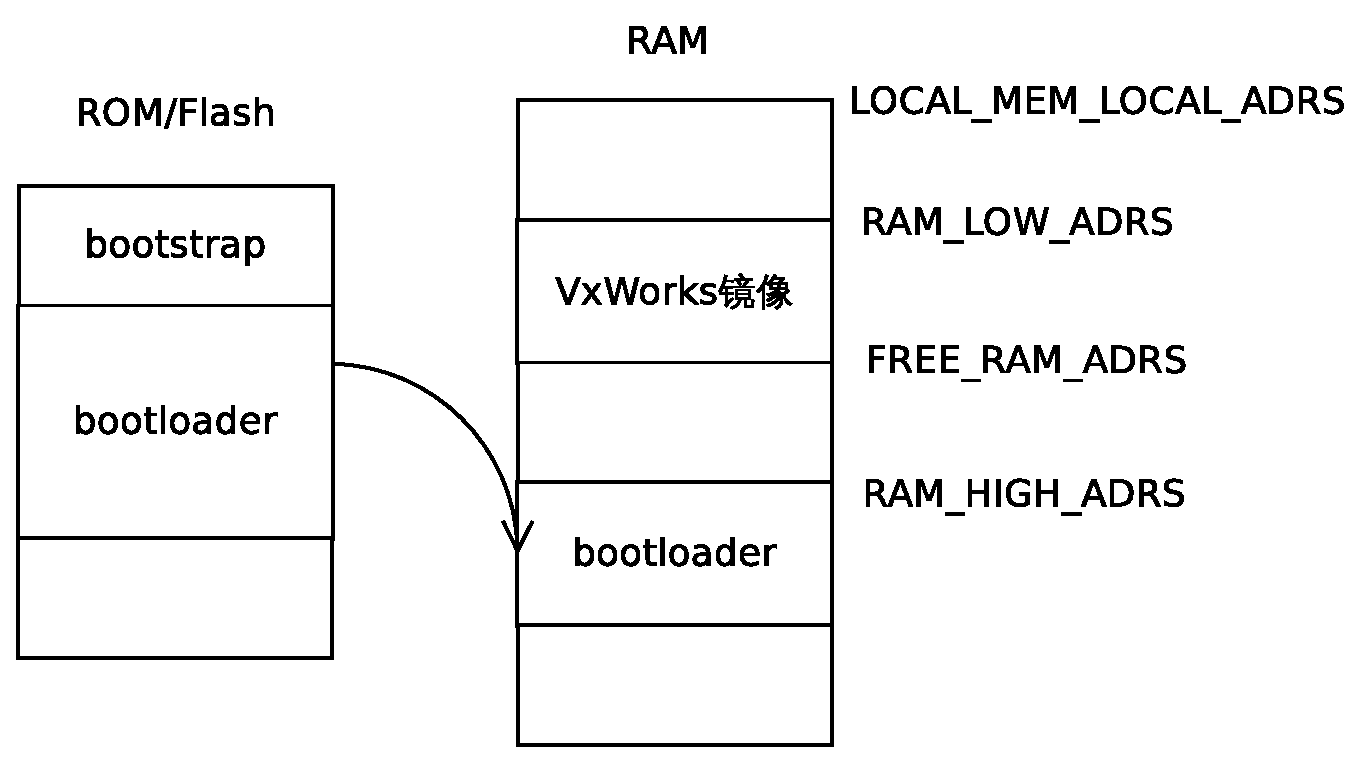
\includegraphics[width=0.68\textwidth]{figure/boot.eps}
    \caption{可加载型VxWorks镜像的启动}
    \label{boot}
\end{figure}

1、系统上电后,执行bootstrap的代码。
该程序进行一些基本的硬件初始化,
并负责将引导程序bootloader加载到
RAM中的RAM\_HIGH\_ADRS处。

2、系统跳转到RAM中,执行bootloader的代码,
该程序进行一些初始化工作之后,
通过网络或其他途径下载可加载型VxWorks镜像,
并加载到RAM中的的RAM\_LOW\_ADRS处。

3、镜像加载完毕后,
跳转到RAM中VxWorks的第一条指令处,
开始进行内核初始化。完成后启动应用程序。


\subsection{可引导型映像的内存布局}

上一条简单介绍了VxWorks可加载型镜像的启动顺序,
并展示了一个简单的、通用的
内存布局。
然而针对特定的体系结构,内存布局有很大的区别。

回顾在xxx中提到的关于ELF文件插入的两个问题:
文件空间与地址空间。
要寻找合适的空闲的地址空间,
我们需要熟悉VxWorks运行中的详细内存布局。

图\ref{ram}是在x86硬件平台下的VxWorsk内存布局的一个简略版本。

\begin{figure}[h!]
    \centering
    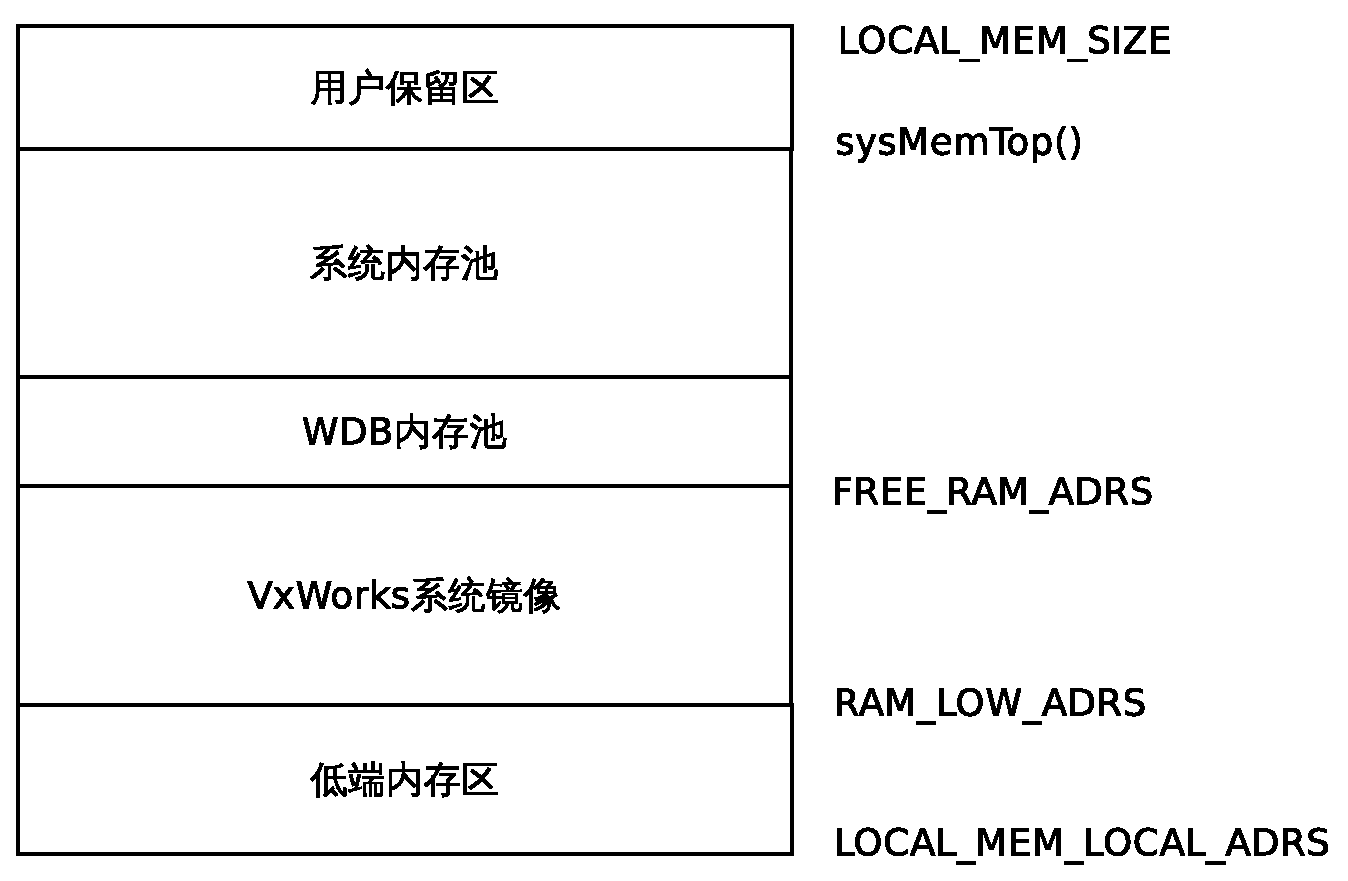
\includegraphics[width=0.68\textwidth]{figure/ram.eps}
    \caption{x86下的VxWorks系统内存布局}
    \label{ram}
\end{figure}

我们的目标是寻找空闲的地址空间,
使得代码能够映射到这一块地址并被执行。
然而,从图中不难看出:
在VxWorks系统镜像的低地址和高地址两个方向,
均有明确的定义和用途。
其中,RAM\_LOW\_ADRS之前
(即.text节之前的地址)的低端内存区,
被用作初始化堆栈。
系统的初始化流程借助这一区域实现函数调用。
而FREE\_RAM\_ADRS之后的地址,
用于WDB内存池。
这两段地址皆有明确的用途,
因此,利用这两段地址空间注入代码是不可行的。
这也就意味着,
我们必须在VxWorks系统映像占据的内存区域中
寻找地址空间进行插入。


\section{环境搭建与配置}

为了把精力集中于二进制层面的插入,
而不是目标版的连接与调试,
我们使用Vmware虚拟机来运行一个VxWorks操作系统。
这意味着我们只需要一台x86的PC就可以完成所有工作。
然而实际上我使用了两个平台:
\begin{itemize}
  \item 一台Linux机器用于修改VxWorks系统映像。
  \item 一台Windows机器用于运行Tornado和Vmware。
\end{itemize}

\subsection{Linux主机}

Linux主机的环境主要为我的修改工作
提供便利的工具,特别是一些GNU实用工具,
例如readelf和objdump。

安装的Linux发行版为Ubuntu 13.10的32位版本,Linux内核版本为3.11。

\subsection{Windows主机与VxWorks虚拟机}

Windows主机的主要任务包含以下几点:

\begin{itemize}
  \item 运行Tornado 2.2,生成引导程序和VxWorks系统镜像。
  \item 运行FTP Server,供目标机下载镜像。
  \item 运行Vmware 9,运行引导程序和VxWorks系统镜像。
  \item 运行Target Sever,用于与目标机通信。
\end{itemize}

图\ref{win}说明了在Windows主机下
各个软件机虚拟机的运行情况。

\begin{figure}[h!]
    \centering
    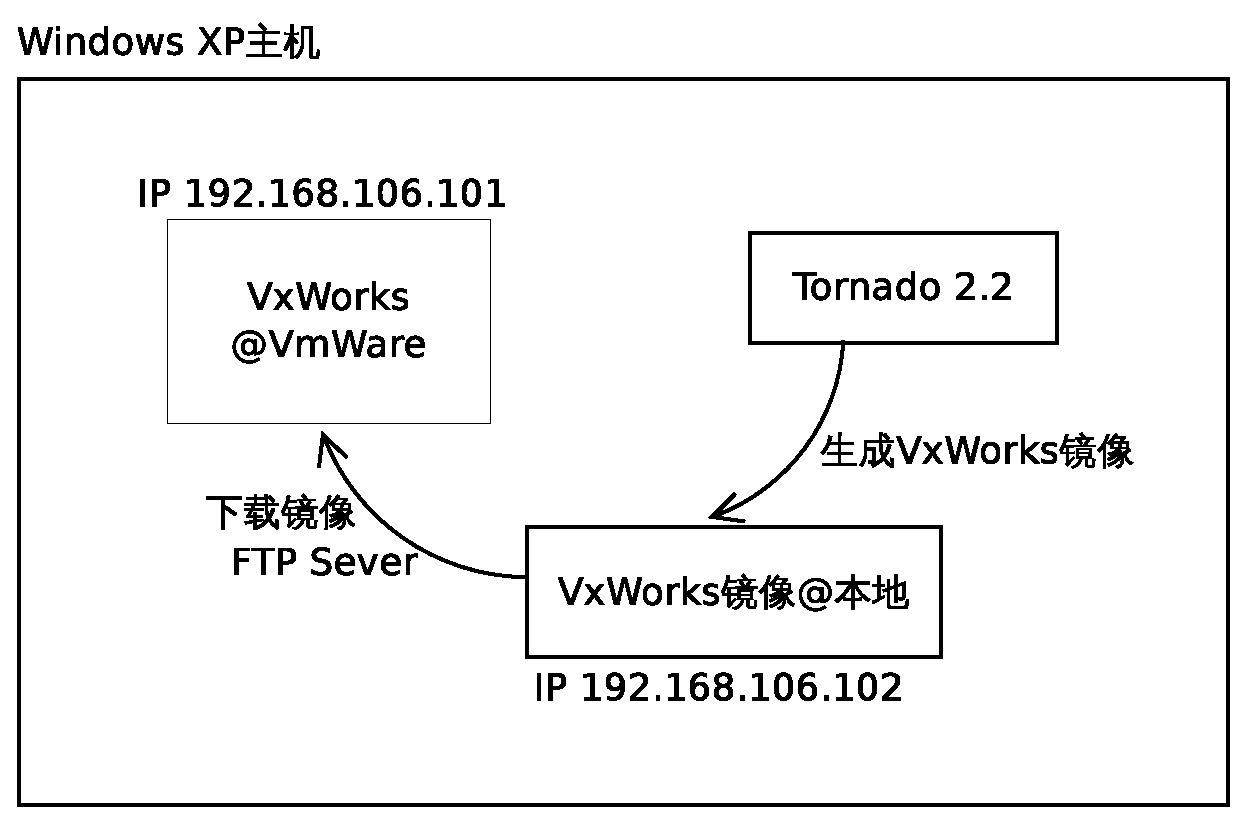
\includegraphics[width=0.68\textwidth]{figure/win.eps}
    \caption{Windows主机下的软件和虚拟机}
    \label{win}
\end{figure}

其中,在Vmware中下载VxWorks镜像,
需要首先载入bootloader,
实现的方式就不再赘述了。
在此我们可以简单地认为Tornado生成了VxWorks镜像,
而在虚拟机中即可通过FTP按照一定的路径找到该镜像
并下载。
因此,我们只需要修改该路径下的镜像文件,
并替换掉原来的文件,
当虚拟机重启后,
就会下载我们修改过的镜像文件。

\section{ELF插入技术在VxWorks中的实践}

本章第一节已经分析了VxWorks启动流程和
内存布局的主要特点。
下面我们具体地来看一下VxWorks系统映像文件。
图\ref{shtandpht}展示了映像文件的
节头表和程序头表,以及他们的映射关系。

\begin{figure}[h!]
    \centering
    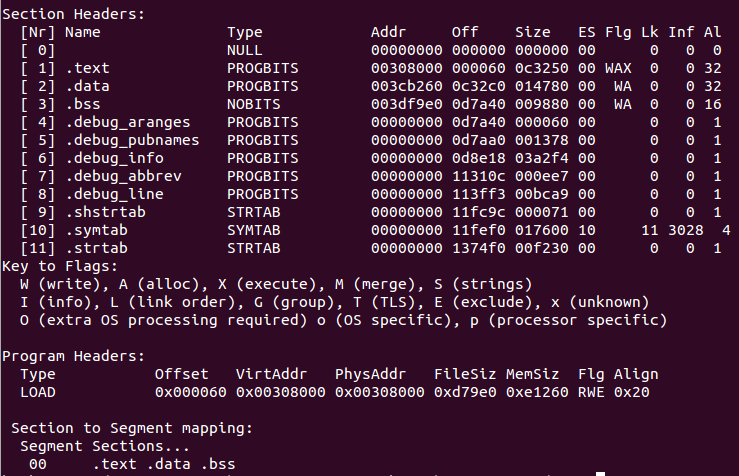
\includegraphics[width=0.68\textwidth]{figure/shtandpht.png}
    \caption{VxWorks系统映像文件的节头表和程序头表}
    \label{shtandpht}
\end{figure}

该文件的布局非常简单,
只有一个可加载段,对应三个节,
分别是text节,data节和bss节。
一般来说,ELF文件中的代码和数据由于分别具有不同的属性
(例如代码节不可写,数据节不可执行),
这两种节会被映射到不同的段来映射,
从而映射到不同的页面,
并在页表中赋予他们不同的属性。
然而VxWorks的做法比较特殊,
代码和数据节映射到一个段,
这也就意味着该段必须同时具有可读可写和可执行三类属性。

这种特殊性对我们的插入有什么影像呢?
回顾一下以前的内容,
要实现代码插入,
最重要的是寻找空闲的地址空间。
由于镜像文件只有一个段,
因此不存在段与段之间因为页对齐而产生的空闲地址空间。
至于节之间的空间就太小了
(例如这里text节和data节的对齐属性都是32字节),
几乎可以忽略不计。
而在这唯一一个段之外的空间,
也早已经被系统分配了专门的用途,
这在本章第一节也讨论过了。

这样看来,似乎我们的插入工作难以取得成功。
然而地址空间就像海绵里的水,
挤挤就会有的。
一方面,我们可以通过nop串实现少量代码的注入。
另一方面,由于数据节也被赋予了执行属性,
因此在数据节的地址空间中写入代码,
理论上也是可行的。
下文分别利用这两种办法实现
对VxWorks系统中的usrAppInit函数的劫持。


\subsection{利用nop串注入代码实现函数劫持}

使用nop串插入代码的原理和技术在2.2.1中有着较为详细的描述。
我们的目标是在VxWorks启动和初始化工作完成后,
执行我们插入的代码,然后跳回。

在Linux下的ELF文件中,
我们可以通过修改ELF头部的入口点地址来
实现劫持。
然而在VxWorks中,
入口点指向的位置是一些初始化函数,
这些函数需要进行一些硬件和内存的初始化工作。
如该劫持入口点,
我们插入的代码很可能无法执行。
系统初始化完成后调用的第一函数,
是usrAppInit,
该函数一般用于启动用户的应用程序。

usrAppInit函数开头部分如图\ref{usr}所示。

\begin{figure}[h!]
    \centering
    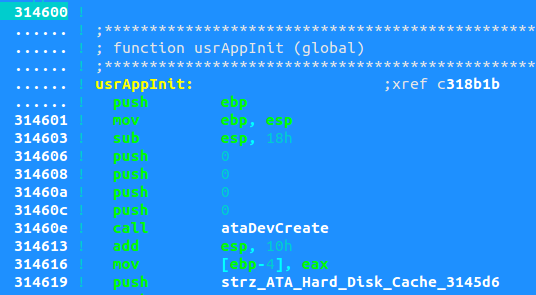
\includegraphics[width=0.64\textwidth]{figure/usr.png}
    \caption{usrAppInit函数的反汇编图示}
    \label{usr}
\end{figure}

我们把usrAppInit前三条指令替换为代码\ref{inj}:

\begin{lstlisting}[
    language={[x86masm]Assembler},
    caption={在usrAppInit开头替换的代码},
    label={inj},
]
push nop_address        ;压入插入代码的起始地址
ret                      ;跳转到nop\_address
\end{lstlisting}


我们使用nop串在合适的位置插入代码\ref{printhello},
\begin{lstlisting}[
    language={[x86masm]Assembler},
    caption={在VxWorks的nop串中插入的代码},
    label={printhello},
]
push ebp
mov ebp,esp
sub esp,0x18            ;补上usrAppInit开头被修改的三条指令
push 0x000a214f
push 0x4c4c4548         ;压入字符串“HELLO!\textbackslash n”的ASCII码
push esp                ;压入字符串的起始地址。  
mov eax,0x00384b80      ;把printf函数的地址放入eax中
call eax                ;调用printf函数
add esp,0x8             ;恢复堆栈
push 0x314606        
ret                     ;返回usrAppInit函数第四条指令处。
\end{lstlisting}


\subsection{通过覆盖数据段插入代码}



\section{利用插入代码实现简单的文件操作监控}
















% !Mode:: "TeX:UTF-8"
%%\chapter{下载}
%%
%%\section{发行版本}
%%
%%发行版本是本模板编写者会不定期更新打包的版本,适合大部分用户使用,
%%优点是相对较为稳定,下载和使用都更方便便捷,
%%缺点是可能不包含一些最新的更新,不过应该足够满足常规毕业设计论文撰写需求。
%%由于本模板仍在开发之中,我们将适时更新本说明文档及相关项目介绍和使用方法,
%%敬请关注后续进展。
%%
%%\section{开发版本}
%%
%%开发版本是通过Git直接clone本模板托管在Github版本库中的最新代码,
%%适合有版本管理工具使用经验和对LaTeX使用较为熟练的用户。
%%优点是包含最新的模板代码,
%%缺点是稳定性无法保证,可能有一些小问题,
%%当然我们很欢迎您通过所有可能的方式将问题反馈给我们。
%%
%%\subsection{下载方法}
%%首先你需要打开准备存放毕业设计论文的目录,
%%通过命令\ref{code-git-clone}即可获取最新的模板代码,
%%需要注意的是这将在当前目录下新建一个名为BUAAthesis的文件夹。
%%\begin{lstlisting}[
%%    language={bash},
%%    caption={git clone},
%%    label={code-git-clone},
%%]
%%git clone git://github.com/BHOSC/BUAAthesis.git
%%\end{lstlisting}
%%
%%\subsection{更新方法}
%%通过命令\ref{code-git-pull}即可实现模板代码的更新,
%%需要注意的是此处可能会出现冲突,相关处理方法将在后续说明。
%%\begin{lstlisting}[
%%    language={bash},
%%    caption={git pull},
%%    label={code-git-pull},
%%]
%%git pull origin master
%%\end{lstlisting}
%%
%%\section{目录结构}
%%
%%本模板项目完整的文件目录结构如下所示:
%%
%%{
%%    \dirtree{%
%%        .1 BUAAthesis/\DTcomment{根目录}.
%%        .2 buaathesis.cls\DTcomment{模板文件}.
%%        .2 buaathesis.bst\DTcomment{参考文献样式}.
%%        .2 sample-bachelor.tex\DTcomment{本科生示例文件}.
%%        .2 sample-master.tex\DTcomment{研究生示例文件}.
%%        .2 data/\DTcomment{数据文件夹}.
%%        .3 abstract.tex\DTcomment{中英文摘要}.
%%        .3 appendix1-faq.tex\DTcomment{附录1,常见问题}.
%%        .3 appendix2-contactus.tex\DTcomment{附录2,联系我们}.
%%        .3 bibs.bib\DTcomment{参考文献文件}.
%%        .3 chapter1-intro.tex.
%%        .3 chapter2-config.tex.
%%        .3 chapter3-download.tex.
%%        .3 chapter4-baisc.tex.
%%        .3 chapter5-usage.tex.
%%        .3 chapter6-implement.tex.
%%        .3 com\_info.tex\DTcomment{通用自定义信息}.
%%        .3 reference.tex\DTcomment{参考文献}.
%%        .3 bachelor/\DTcomment{本科生专属文件}.
%%        .4 assign.tex\DTcomment{任务书}.
%%        .4 bachelor\_info.tex\DTcomment{本科生专属信息}.
%%        .4 thanks.tex\DTcomment{致谢页}.
%%        .3 master/\DTcomment{研究生专属文件}.
%%        .4 back1-achievement.tex\DTcomment{附页1,取得成绩}.
%%        .4 back2-thanks.tex\DTcomment{附页2,致谢}.
%%        .4 back3-aboutauthor.tex\DTcomment{附页3,关于作者}.
%%        .4 denotation.tex\DTcomment{主要符号对照表}.
%%        .4 master\_info.tex\DTcomment{研究生专属信息}.
%%        .2 figure/\DTcomment{图片存放路径}.
%%        .3 buaamark.eps\DTcomment{北航Logo,用于页眉}.
%%        .3 buaaname.eps\DTcomment{北航校名,用于首页}.
%%        .3 fgbt.jpg\DTcomment{北航未来花园Logo,用于测试}.
%%        .2 Makefile\DTcomment{Linux下辅助脚本}.
%%        .2 msmake.bat\DTcomment{Windows下辅助脚本}.
%%        .2 README.md\DTcomment{Github项目说明}.
%%        .2 .gitignore\DTcomment{Git版本管理配置文件}.
%%    }
%%}
